\documentclass[numbers=noenddot,12pt,a4paper]{scrartcl}
\usepackage[greek,ngerman]{babel}
\usepackage[T1]{fontenc}
\usepackage[utf8]{inputenc}
\usepackage{fullpage}
\usepackage{libertine}
\usepackage{ziffer}
\usepackage{graphicx}
\usepackage{units}
%\usepackage{wasysym}
\usepackage{amsmath}
\usepackage{amssymb}
\usepackage{wrapfig}
\usepackage{esint}
\usepackage{float}
\usepackage{wrapfig}
\usepackage[font=small]{caption}
\usepackage{subcaption}

\renewcommand{\thefigure}{Abb. \arabic{figure}}

\captionsetup[wrapfigure]{name=}
\captionsetup[figure]{name=}
\newcommand{\degree}{^\circ}
\newcommand{\diff}{\textnormal{d}}
\newcommand{\tenpo}[1]{\cdot 10^{#1}}
\newcommand{\greek}[1]{\greektext#1\latintext}
\newcommand{\ix}[1]{_\text{#1}}
\newcommand{\imag}{\mathbf{i}}

\title{Protokoll: Digitale Schaltungen}
\author{Tom Kranz, Philipp Hacker}
\date{\today}

\begin{document}
%\setcounter{page}{2}
%\setcounter{section}{1}
\maketitle
\vspace*{\fill}
\tableofcontents
\vfill
\newpage
\section{Schaltskizzen}
\begin{figure}[H]
\centering
%TODO Bild einfügen
\caption{IC SN 7400 bzw. SN 74HCT00} \label{img:ic}
\end{figure}
\section{Durchführung}
\subsection{Versuchsaufgabe 1}
Hierbei wurden die beide Eingänge eines NAND-Gatters mit einem Signal $U\ix{x}$ beschaltet. Zuerst wurde der Verlauf des Ausgangssignals $U\ix{y}$ bei den quasistatischen Variationen $U\ix{x}=0\rightarrow\unit[5]{V}$ und $U\ix{x}=5\rightarrow\unit[0]{V}$ mittels Multimetern gemessen Anschließend wurde für das Eingangssignal ein systemeigener Rechteckimpuls der Frequenz $1$ bzw. $\unit[10]{MHz}$ eingesetzt. Systemeigen bedeutet hierbei, dass ein Gatter zwischen ursprünglicher Spannungsquelle und Eingang des Messgatters geschaltet war. Der Rechteckimpuls hatte eine Peak-to-Peak-Spannung von $\unit[5]{V}$ mit einem Offset von $\unit[2,5]{V}$. Ein- und Ausgangssignal wurden zeitsynchron oszillographiert.
\subsection{Versuchsaufgabe 2}
Für 2 unterschiedliche ICs (siehe \ref{sec:gerät}) wurde die Verlustleistung in Abhängigkeit von der Frequenz des ansteuernden systemeigenen Rechteckimpulses gemessen. Dabei wurde die Stromaufnahme mit freien Gattern, d.h. alle Gatter sind ohne Ein- bzw. Ausgangssignal, und mit beschalteten Gattern gemessen.
\subsection{Versuchsaufgabe 3}
Wie in \ref{img:ic} gezeigt, können beliebig Ein- bzw. Ausgänge von Gattern in einem IC miteinander verschaltet werden. Hierbei sollte nun, nacheinander für die ICs aus \ref{sec:gerät}, bis zu 3 Gatter in Reihe geschaltet werden. Gemessen wurde die Ausgangsspannung des 1. Gatters, welches für jede Schaltung mit einem High $U\ix{H}$ und einem Low $U\ix{l}$ auf beiden Eingängen angesteuert wurde. \\
Für die Schaltung mit keinem nachgeschalteten Gatter wurden die Eingänge \textbf{1} und \textbf{2} zusammengelegt und, wie in allen anderen Schaltungen auch, der Ausgang \textbf{3} gemessen. Mit einem Gattern wurde der Ausgang \textbf{3} zusätzlich auf die Eingänge \textbf{4} und \textbf{5} gelegt. Für 2 Gatter wurde das Signal aus \textbf{3} wiederum auf \textbf{9} bzw. \textbf{10} geschaltet. Schließlich wurde für 3 Gatter das Ausgangssignal aus \textbf{3} auf alle Eingänge des ICs weitergegeben (für Nummerierung siehe \ref{img:ic}).
\subsection{Geräte} \label{sec:gerät}
Die verwendete Versuchsplatine ist "`Logisches Gatter"'. Die Betriebsspannung und die verschiedenen Eingangs-Gleichspannungen lieferte das Stromversorgungsgerät \textsc{Tektronix PS 280}, Rechtecksignale wurden mit dem Funktionsgenerator \textsc{Tektronix AFG 3022B} erzeugt. Die Gleichspannungen wurden mit dem Multimeter \textsc{VOLTCRAFTplus VC 920} gemessen, Oszillogramme und Signalverläufe mit dem Oszilloskop \textsc{Hameg HM1508-2} erstellt bzw. betrachtet.
\subsection{Oszillogramme}
\subsubsection{Versuchsaufgabe 1}
\begin{figure}[H]
\begin{subfigure}[b]{0.48\textwidth}
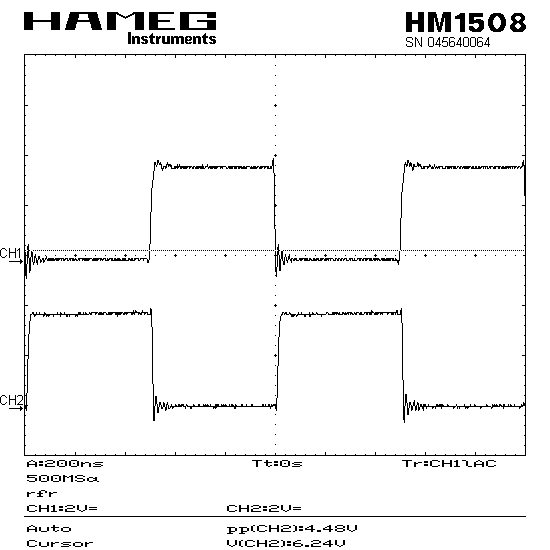
\includegraphics[width=\textwidth]{scr16.png}
\caption{$f=\unit[1]{MHz}$}
\end{subfigure}
\begin{subfigure}[b]{0.48\textwidth}
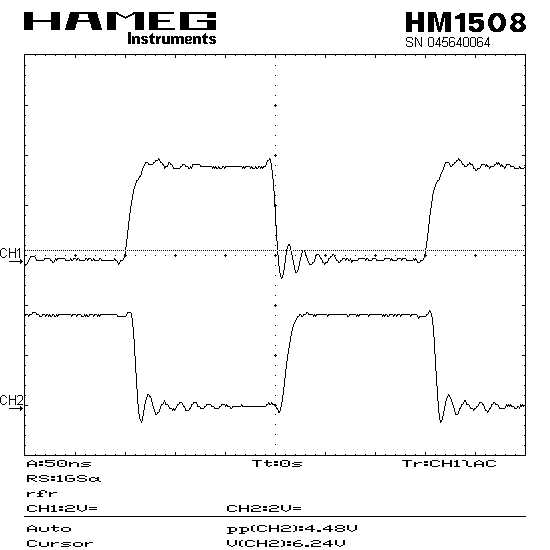
\includegraphics[width=\textwidth]{scr17.png}
\caption{$f=\unit[10]{MHz}$}
\end{subfigure}
\caption{zeitsynchrone Ein- und Ausgangssignale (systemeigen, Rechteckimpuls)}
\end{figure}
\section{Auswertung}
\subsection{Versuchsaufgabe 1}

\subsection{Versuchsaufgabe 2}
\subsection{Versuchsaufgabe 3}
\section{Anhang}
Die originalen Messwert-Aufzeichnungen liegen bei.
\end{document}